\documentclass[a4paper,12pt]{article}

\usepackage[utf8x]{inputenc}
\usepackage[T2A]{fontenc}
\usepackage[english, russian]{babel}

% Опционно, требует  apt-get install scalable-cyrfonts.*
% и удаления одной строчки в cyrtimes.sty
% Сточку не удалять!
% \usepackage{cyrtimes}

% Картнки и tikz
\usepackage{graphicx}
\usepackage{tikz}
\usetikzlibrary{snakes,arrows,shapes}


% Некоторая русификация.
\usepackage{misccorr}
\usepackage{indentfirst}
\renewcommand{\labelitemi}{\normalfont\bfseries{--}}

% Увы, поля придётся уменьшить из-за листингов.
\topmargin -1cm
\oddsidemargin -0.5cm
\evensidemargin -0.5cm
\textwidth 17cm
\textheight 24cm

\sloppy

% Оглавление в PDF
\usepackage[
bookmarks=true,
colorlinks=true, linkcolor=black, anchorcolor=black, citecolor=black, menucolor=black,filecolor=black, urlcolor=black,
unicode=true
]{hyperref}

% Для исходного кода в тексте
\newcommand{\Code}[1]{\texttt{#1}}


\title{Отчёт по лабораторной работе \\ <<Система доменных имён>>}
\author{(Фроловского Алексея Вадимовича)}

\begin{document}

\maketitle

\tableofcontents

\section{Настройка системы DNS}

\subsection{Топология сети}

Топология сети и использыемые IP-адреса показаны на рис.~\ref{fig:network}.

\begin{figure}
\centering
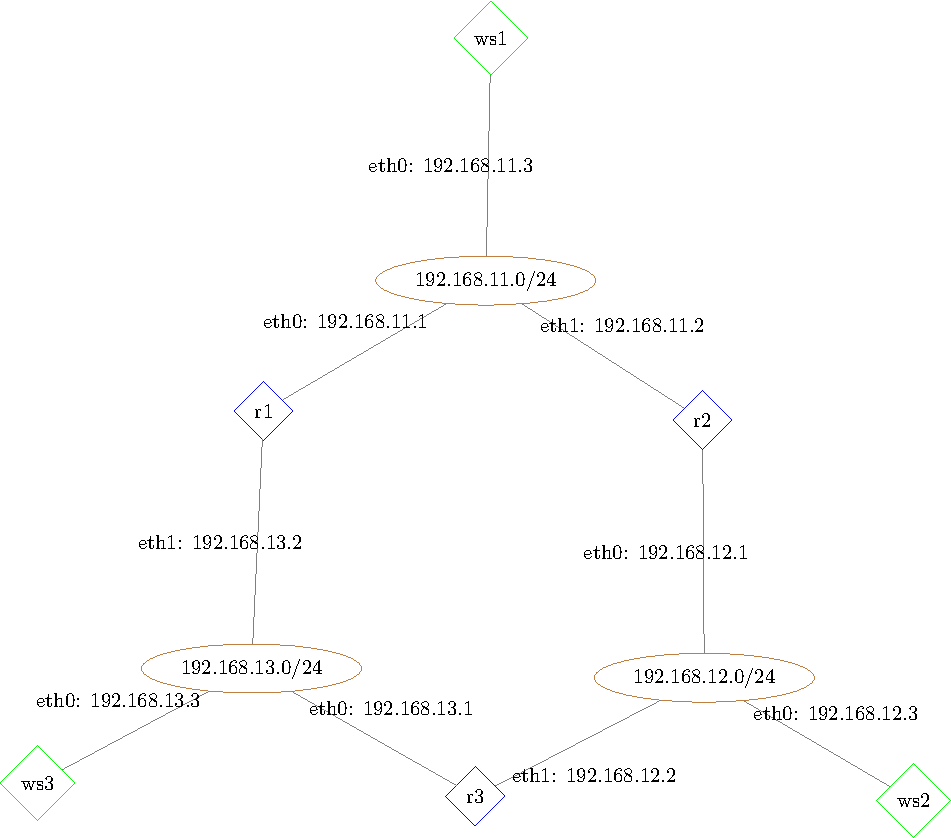
\includegraphics[width=\textwidth]{includes/network_gv.pdf}
\caption{Топология сети}
\label{fig:network}
\end{figure}

\subsection{Структура службы доменных имён}

Структура авторитетных серверов доменных имён показана на рис.~\ref{fig:dns}.

\begin{figure}
\centering
\includegraphics[width=\textwidth]{includes/dns_gv.pdf}
\caption{Структура службы доменных имён}
\label{fig:dns}
\end{figure}

\subsection{Прочие настройки}

Кеширующие DNS-серверы
\begin{itemize}
\item ... ;
\item ...
\end{itemize}

Развёрнутые SMTP-серверы и используемые ими кеширующие DNS-серверы.
\begin{itemize}
\item ... использует сервер на ... ;
\item ...
\end{itemize}


\section{Проверка настройки службы доменных имён}

\subsection{Проверка настройки записи типа ... для домена ...}

(по цепочке опрашиваем с корневого сервера ручками)

\begin{verbatim}
первый вывод dig
\end{verbatim}

\begin{verbatim}
второй вывод dig
\end{verbatim}

...

Итоговая проверка: опрашиваем кеширующий DNS-сервер.

\begin{verbatim}
Здесь вывод dig при опросе кеширующего сервера.
\end{verbatim}

\begin{verbatim}
Здесь вывод ping для искомого имени.
\end{verbatim}

\subsection{Проверка настройки записи типа ... для домена ...}

Повторяем далее.

\section{Проверка работы почтовой системы}

\subsection{Проверка MX-записи для домена ...}

С узла ... отправили письмо на локальный SMTP-сервер для адресата с адресом .....

\begin{verbatim}
Сюда нужно поместить лог работы с SMTP-сервером.
\end{verbatim}

На машине с доменным именем ... появилось доставленное письмо.
\begin{verbatim}
Результат cat /var/mail/...
\end{verbatim}

Таким образом, доменная запись типа MX для домена ... настроена верно.

\subsection{Проверка MX-записи для домена ...}

(повторить для всех SMTP-серверов)

\end{document}
